%%
%% This is file `mcmthesis-demo.tex',
%% generated with the docstrip utility.
%%
%% The original source files were:
%%
%% mcmthesis.dtx  (with options: `demo')
%%
%% -----------------------------------
%%
%% This is a generated file.
%%
%% Copyright (C)
%%     2010 -- 2015 by Zhaoli
%%     2014 -- 2016 by Liam 
%%     2017 -- 2019 by Xuehan
%%
%% This work may be distributed and/or modified under the
%% conditions of the LaTeX Project Public License, either version 1.3
%% of this license or (at your option) any later version.
%%
%% This work has the LPPL maintenance status `maintained'.
%%
%% The Current Maintainer of this work is Xuehan.
%%
\documentclass{mcmthesis}
\bibliographystyle{IEEEtran}
\mcmsetup{CTeX = false,   % 使用 CTeX 套装时,设置为 true
        tcn = 2002134, problem = D,
        sheet = true, titleinsheet = true, keywordsinsheet = true,
        titlepage = true}
\usepackage{palatino}
\usepackage{mwe}
\usepackage{graphicx}
\usepackage{subcaption}
\usepackage{float}
\usepackage{multirow}
\usepackage{indentfirst}
\usepackage{gensymb}
\usepackage[ruled,lined,commentsnumbered]{algorithm2e}
\usepackage{geometry}

\begin{document}
\linespread{0.6} %%行间距
\setlength{\parskip}{0.5\baselineskip} %%段间距
\title{ti}

\date{\today}
	\begin{abstract}

	
		\begin{keywords}
		
		\end{keywords}
	\end{abstract}

\maketitle

\tableofcontents

\newpage

\section{Introduction}
\subsection{Problem Background}
	Football is one of the most well-known sports activities in the world.  The standard system of an 11-man football game is one goalkeeper and 10 players from each of the two teams. There are a total of 22 players who fight, defend and attack on the rectangular grass court.  The game scores by shooting the ball into the opponent's goal. When the game is over, the team with the most points wins.

	\begin{figure}[h]
		\centering
		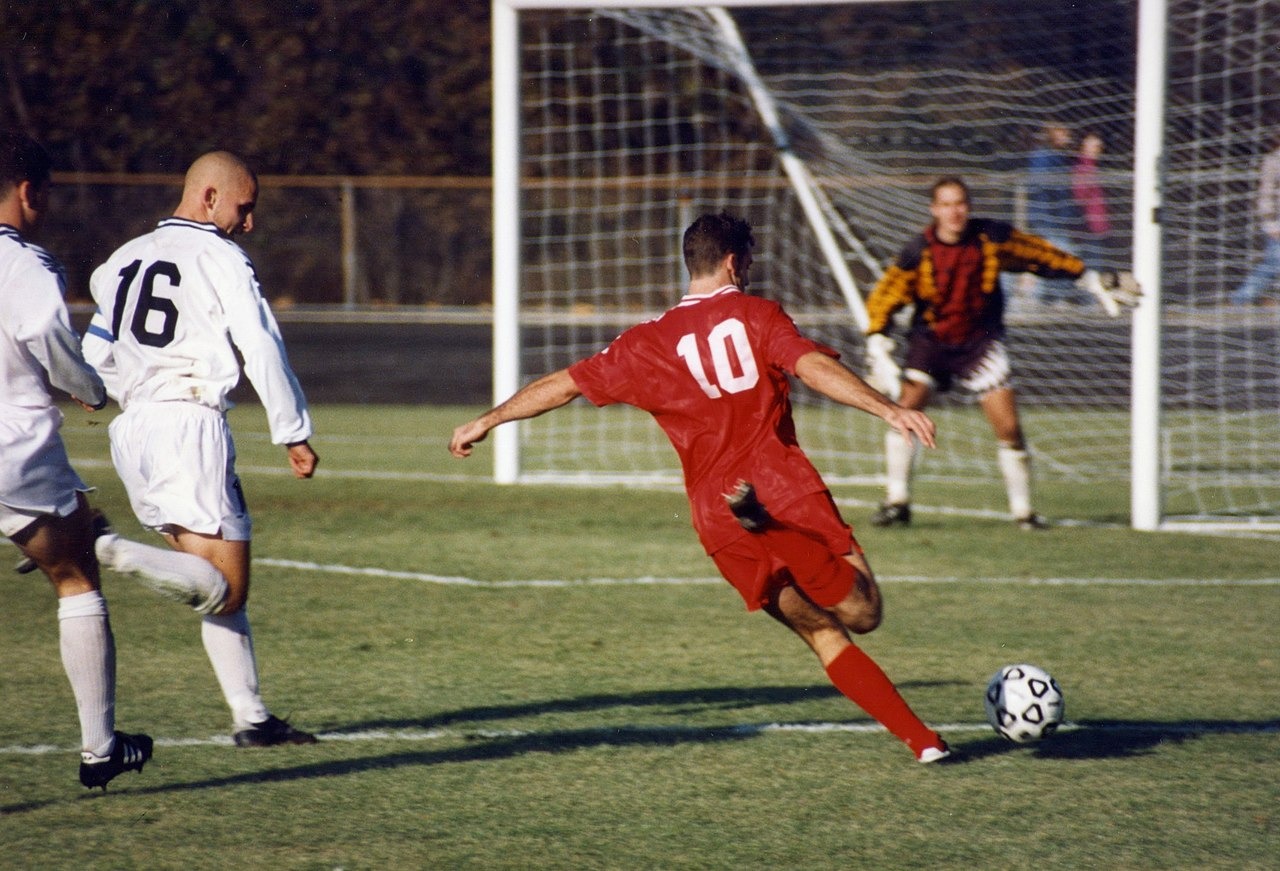
\includegraphics[width=0.75\textwidth]{figures/football.jpg}
		\caption{A Football Game~\cite{Wiki_Football}}
		\label{fig:football}
	\end{figure}

	As we all know, football is a sport that requires intense teamwork.  For it can show the importance of teamwork spirit more than superb personal ability.  Passing, as an offensive means that requires the cooperation of various players to play the biggest role, is just an important manifestation of the team spirit of football.  Therefore, to study the important role of teamwork in football, you can start by studying the passing network in football.

	Our goal is to build a network model to simulate the Huskies' passing network and study it.  Meanwhile, it is necessary to extract some representative parameters from the constructed network model.  Through the study of such parameters, we can accurately understand the team collaboration ability and structural characteristics of this team.
\subsection{Our Work}
	In this paper, we successfully built the Huskies' passing network model.  On the basis of this network model, we obtained some important parameters. In this way, we analyzed the team collaboration ability of the Huskies players, and offered some suggestion for its future structural strategy.

	In Section 2, we state some basic assumptions.  Section 3 contains the nomenclature used in the statement of our model.  Section 4 provides sufficient details about our network model.  Section 5 carries on the simulation experiment and analysis to our proposed model.  Section 6 provides some advice on its structural strategies for the Huskies.  Finally, we further analyze the sensitivity, advantages and disadvantages of our model in Section 7, and we obtain some conclusions on how to improve the teamwork spirit of general teams in Section 8.
\section{Assumptions}
	Our model is based on these following basic assumptions:
	\begin{enumerate}
		\item The average position of a player over a period of time is equivalent to the average of the position of the player in all events that occurred during that period.
		\item We consider a dyadic configuration tight if this kind of dyadic configuration appears far more often than others.  The same is true for triadic configurations.
	\end{enumerate}
\section{Nomenclature}
	Symbols that our model mainly uses are listed in Table \ref{tab:Nomen}.  Other symbols that are used only once will be described in the following chapters.
	\begin{table}
    	\centering
    	\caption{Nomenclature}
		\label{tab:Nomen}
		\begin{tabular}{c c}
			\hline	
				Symbol & Definition\\
			\hline
				$\textbf{A}$ & Football passing matrix\\
				$\textbf{B}$ & Adjacency matrix\\
				$G$ & Undirected graph representing the football passing network\\
				$p_{i}$ & The \emph{i}th player in Huskies\\
				$p_{ij}$ & Number of passes from player $i$ to player $j$\\
				$\langle$$X$$\rangle$ & The x-coordinate of the network centroid\\
				$\langle$$Y$$\rangle$ & The y-coordinate of the network centroid\\
				$D$ & The dispersion of the position of the players around the network centroid\\
				$r$ & The advance speed\\
			\hline
   	 	\end{tabular}
	\end{table}

\section{The Basic Model}
	In this section we will discuss our network model in detail.  First of all, we will begin with the establishment of our network model.  Then we will use our model to identify some patterns of the network.  Finally, we will also investigate the indicators of teamwork. 
\subsection{Build of the Network}
	First of all, we define Huskies' football passing matrix $\textbf{A}$.  When the number of players who have played is $n$, $\textbf{A}$ is a square matrix of $n \times n$, which is defined as:
	\begin{equation}\label{eq:Mat_A}
		a_{ij} =
		\begin{cases}
			p_{ij}& \text{$i \neq j$}\\
			0& \text{$i = j$}
		\end{cases}
	\end{equation}
	In this way, we obtain an asymmetric square matrix of order $n$.  Next, on this basis, we try to build an undirected graph model to describe the team's passing network.  But as we have mentioned before, the adjacency matrix of an undirected graph is a symmetric matrix, while the football passing matrix $\textbf{A}$ we constructed is asymmetric.  Therefore, we need to construct a symmetric adjacency matrix $\textbf{B}$ using this asymmetric passing matrix $\textbf{A}$.  To achieve this, we define $\textbf{B}$ as the sum of $\textbf{A}$ and the transposed matrix of $\textbf{A}$, that is to say, for each element $b_{ij}$ in B, the following formula is satisfied:
	\begin{equation}
		\label{eq:Mat_B}
		b_{ij} = a_{ij} + a_{ji}
	\end{equation}
	Now we can easily find that $\textbf{B}$ is equal to its transpose matrix.  Hence $\textbf{B}$ is a symmetric matrix.

	After getting $\textbf{B}$, we can continue to study the undirected graph $G$.  From the previous definition of the adjacency matrix, it can be seen that the nodes in this undirected graph represent the Huskies players, and the edges represent interactions between players.  For quantitative research, we define the weight of node $i$ in the undirected graph $G$ as the sum of the number of passes and catches by player $i$, and the weight of edge $E (i, j)$ is defined as the sum of the number of passes from player $i$ to player $j$ and the number of passes from player $j$ to player $i$.
	
	In order to have an intuitive understanding of the football passing network, we can draw this undirected graph on a schematic diagram of a football field.  Among them, circles represent nodes, and straight lines connecting circles represent edges.  For a node, the larger its size and the darker its color, the greater the weight of the node.  For an edge, the thicker its thickness and the darker its color, the greater the weight of the edge.  In addition, in order to gain a clear understanding of the formation and other factors of this team, we plot the nodes on the represented player's the average position in the studied period.  In this way, we obtain a schematic diagram which can intuitively reflect the football passing network.  Figure \ref{fig:playground} is an example by us.
	
	\begin{figure}[h]
		\centering
		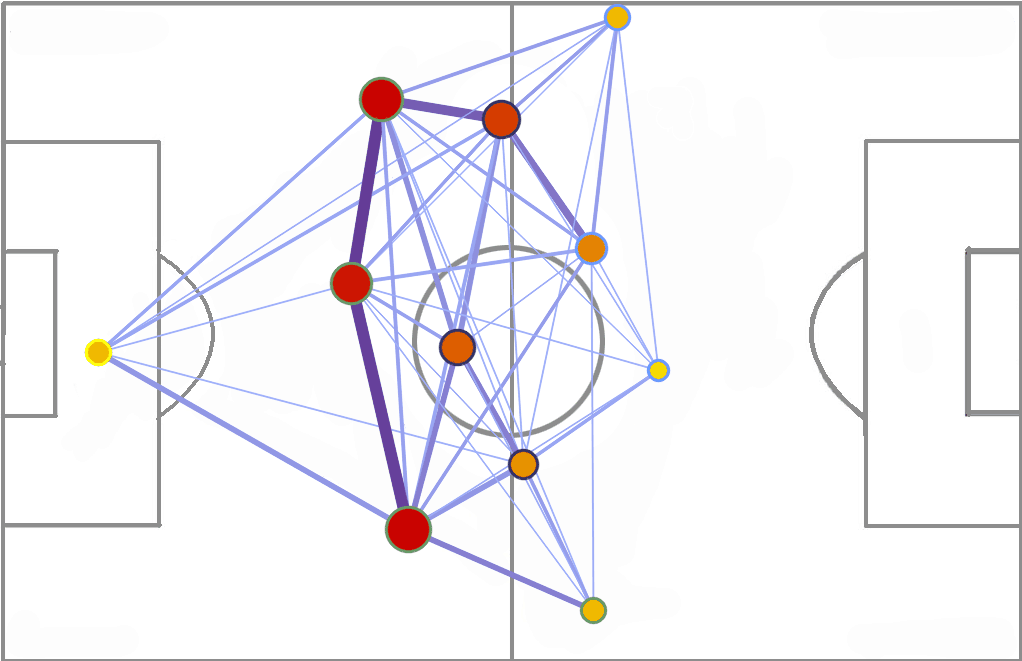
\includegraphics[width=\textwidth]{figures/playground.png}
		\caption{An Example of the Football Passing Network}
		\label{fig:playground}
	\end{figure}
\subsection{Identify Network Patterns}
	After establishing the football passing network, we will use this model to identify some special patterns of Huskies' network.  In the following chapters, we will investigate Huskies' continuous football passing chain, network centroid and advance speed to identify its patterns on multiple scales. 
\subsubsection{Continuous Football Passing Chain}
	Just as we have stated in assumption 2, when players in a dyadic or triadic configuration continuously pass each other far more frequently than they do with other players in the team, we consider this configuration tight.  Therefore, when investigating the tightness of such configurations, we need to study the behavior of continuous passing between players.  For this reason, we construct a continuous football passing chain as a tool to study this behavior according to the football passing network.

	In football games, passing is a very continuous activity.  It can be said that before occasion like shooting, out of bounds or the football is intercepted by the opposing player occurs, the passing can build a transitive binary relationship between our players.  Therefore, we can use this characteristic to construct a continuous football passing chain, which is continuous and transitive.  The general construction method is: According to the data in passingevents, we record the process of continuous passing of football between Huskies players with a linked chain.  This chain will continue until disruptive occasions such as shooting, out of bounds or the football is intercepted by the opponent occur.  In this way, we get a chain that records the continuous passing of the Huskies players.

	From the continuous football passing chains, we can easily identify those tight dyadic and triadic configurations.  For example, if we want to identify a dyadic configuration, we can study these chains based on the characteristics that players in this dyadic configuration pass each other more frequently.  We can just number these two players we are studying as 0 and 1. In this way, there will be a large number of fragments like"0 - 1 - 0 - 1" or "0 - 1 - 0 - 1 - 0" in the continuous football passing chain.  If we want to identify those triadic configurations that are tight, we can just look for those fragments such as "0 - 1 - 2 - 1" or "0 - 1 - 2 - 0" from the continuous football pass chain.  Obviously, we can make similar judgments about multiple configurations.  Therefore, it will be convenient for us to find out which kind of configuration appears most.
\subsubsection{Network Centroid And Advance Speed}
	Studying the network centroid and advancing ratio of Huskies' football passing network will display the spatial features of the network better~\cite{First}.  In this section, we will study the coordinates of the network centroid of the football passing network constructed previously, the dispersion of the position of Huskies players around the network centroid, and the advance speed.

	We first study the coordinates of football passing network centroid.  According to the description of coordinates in readme, the x-coordinate on the field is oriented from the perspective of the team that is attacking, where 0 indicates the attacking team's own goal, and 100 indicates the oppositing team's goal.  While for y-coordinate, 0 indicates the attacking team's left-hand side, and 100 indicates its right-hand side.  We define the coordinates of a pass $(x_{i}, y_{i})$ as the average of the origin and destination positions.  Furthermore, we define the coordinates of the network centroid over a period of time as the average coordinates of all passes during that period.  It can be expressed as the following formula: 
	$$\langle X \rangle=\sum_{i=1}^n\frac{1}{n} x_{i}$$
	$$\langle Y \rangle=\sum_{i=1}^n\frac{1}{n} y_{i}$$
	The change of the network centroid coordinates over time can clearly reflect the overall movement tendency of the entire team during this time.  Besides,regardless of the length of the research period, it can always convey some information about the spatial features of the network.

	Then we continue to study the dispersion of the position of Huskies players around the network centroid.  Similarly, we define the dispersion of the position of Huskies players around the network centroid over a period of time $D$ as the variance between the average position of each player and the position of the network centroid during this period.  It can show how dispersed the team is on the court during this time.  Hence it can also reflect the degree of team control over the playing field during this time.  The greater the degree of dispersion, the stronger the team's ability to control the field.

	Finally, we define the team's advance speed over a period of time $r$ as the ratio of the sum of the absolute values ​​of the lateral displacement and the sum of the absolute values ​​of the longitudinal displacement of all its passes during that period. Its formula is:
	$$r=\frac{|\Sigma \Delta x|}{|\Sigma \Delta y|}$$
	The advance speed indicates the team's passing direction.  Besides, it can also reflect the team's movement tendency and offensiveness during this period.
\subsection{Identify Teamwork Indicators}
\section{Implementation}
	In this section, we will analyze network patterns and teamwork indicators of Huskies' football passing network by studying the data given in problem. 
\subsection{Network Patterns}
	We will search for the dyadic and triadic configurations that often appear by studying continuous football passing chain first.  After that, we will analyze the spatial features of Huskies by investigating the network centroid and advance speed.
\subsubsection{Dyadic And Triadic Configuration}
	In a directed graph, we call different connection methods in dyadic and triadic configurations as different mode motifs.  It is obvious that dyadic and triadic configurations both have multiple different mode motifs~\cite{Second}.  In order to make statistics on these different mode motifs and determine which one appears most, we need to further visualize the continuous football passing chain.  Our idea is to reconstruct the continuous football pass chain into the form of a directed graph, so that the number of occurrences of motifs can be identified from the graph according to different directed graphs corresponding to different mode motif.

	First, we store the data given in the problem into a continuous football passing chain in the form of a linked list.  After that, we correspond the continuous football pass chain with the players to construct a directed continuous football pass graph.  Now, we can identify those frequently appearing mode motifs from these directed graphs.  We have made statistics on the occurrence of different mode motifs, and the results are shown in the following figures.

	\begin{figure}[h]
		\centering
		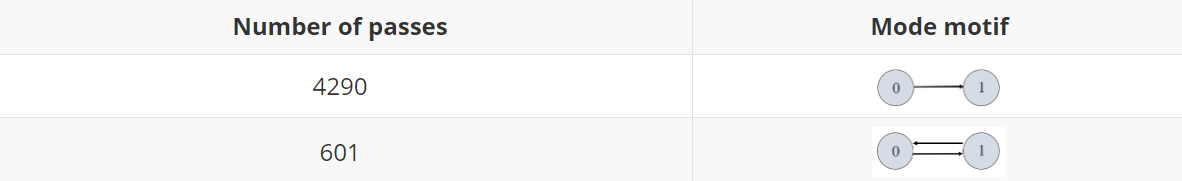
\includegraphics[width=0.75\textwidth]{figures/motif2.png}
		\caption{Statistics on the Occurrences of Different Mode Motifs of Dyadic Configuration}
		\label{fig:motif2}
	\end{figure}
	\begin{figure}[h]
		\centering
		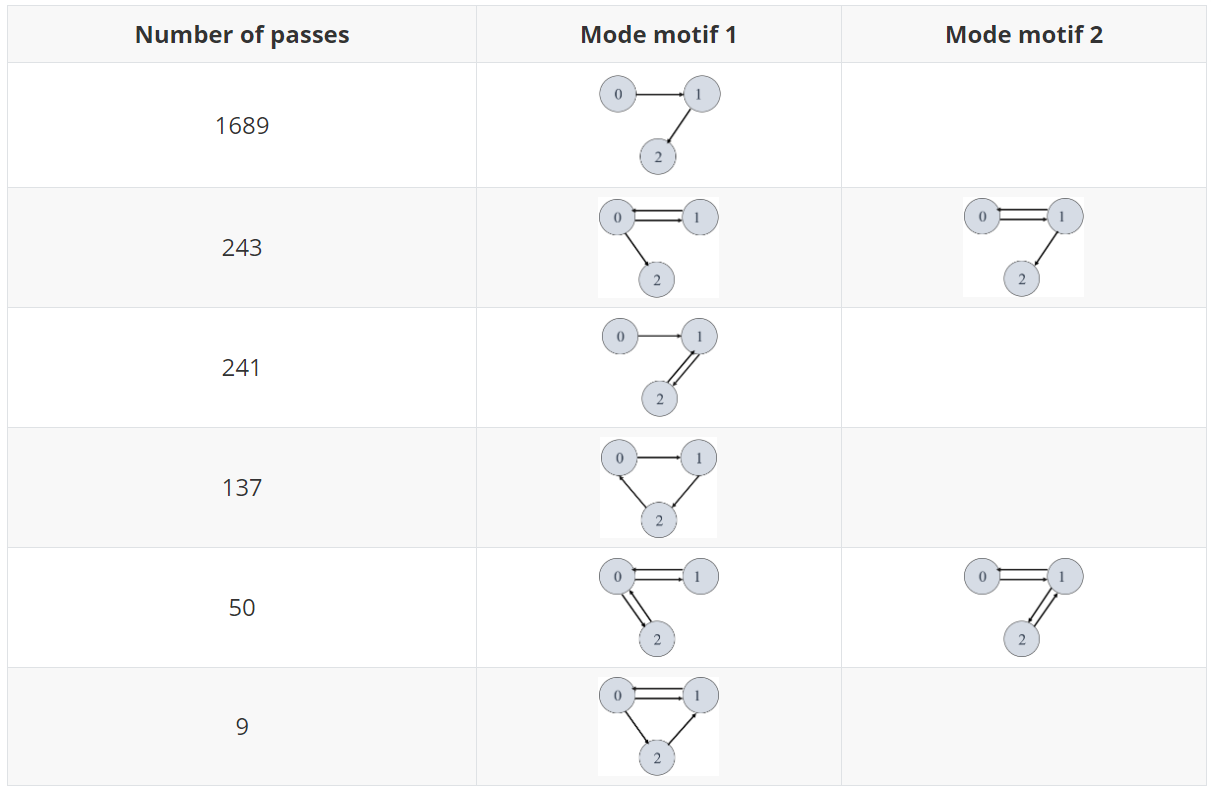
\includegraphics[width=0.75\textwidth]{figures/motif3.png}
		\caption{Statistics on the Occurrences of Different Mode Motifs of Triadic Configuration}
		\label{fig:motif3}
	\end{figure}
	
	We ignore the naive case that appears first in each configurations.  From figure \ref{fig:motif2} and figure \ref{fig:motif3}, we can intuitively see that in the case of dyadic configurations, the Huskies often use "0 - 1 - 0" and "0 - 1 - 0 - 1" mode motifs for passing.  For the triadic cases, it often uses "0 - 1 - 0 - 2", "0 - 1 - 2 - 1" and "0 - 1 - 2 - 0" mode motifs.  Compared with the longer dyadic and triadic chains, these passing mode motifs have more flexibility, but  can still be improved.

	In addition to dyadic and triadic configurations, we also select the case where the number of players is 4 as a representative of multiple configurations, and make statistics on the occurrence of its different mode motifs.  But because its number of mode motifs is far more than dyadic and triadic configurations, we put it in the appendices.
\subsubsection{Spatial Features}
	In this part, we have calculated the coordinates of the network centroid, the dispersion of the position of the players around the network centroid and advance speed of the Husky team's football passing network.  In order to make the results more general, we have calculated both the changes of these statistics per minute in a game, and the changes of these quantities in different games throughout the season.  Here are our statistics.

	We will analyze the statistics of a game first. Figure \ref{fig:game} shows the statistics of Huskies in a certain game.  From the coordinates of the network centroid, it can be seen that the Huskies players were closer to the opponent's goal in the second half, reflecting their fierce offensive in the second half.  It is clear by investigating the dispersion of the position of the players around the network centroid that the players are more concentrated in the second half, which confirms the opinion that the offensive in the second half is more fierce.  Judging from the advance speed, as the game progresses, the movement of the Huskies players is more inclined to go straight to the goal instead of a roundabout movement, which also confirms the previous opinion.
	\begin{figure}[h]
		\centering
		\begin{subfigure}[b]{0.5\textwidth}
			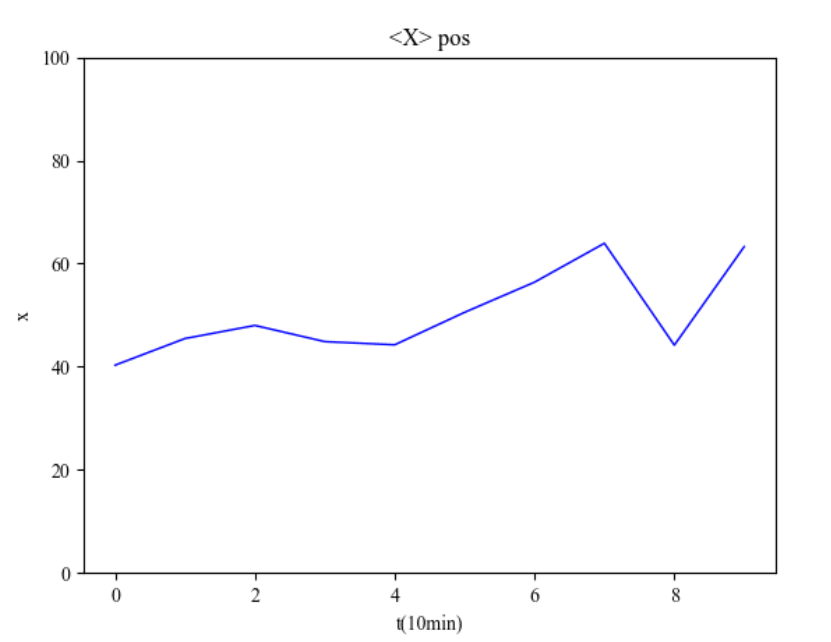
\includegraphics[width=\textwidth]{figures/xc1.png}
			\caption{The X-coordinate of the Network Centroid.}
			\label{fig:x1}
		\end{subfigure}%
		\begin{subfigure}[b]{0.5\textwidth}
			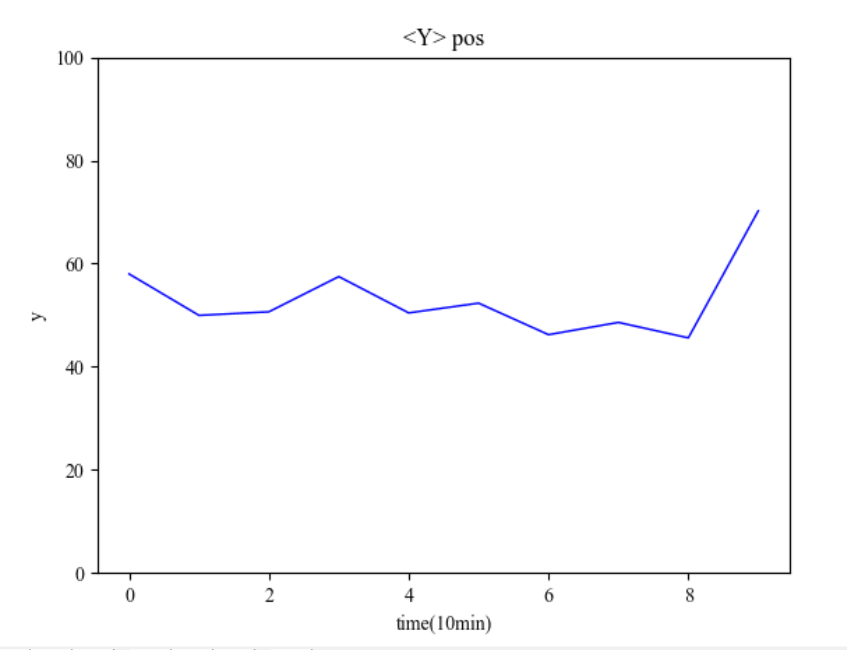
\includegraphics[width=\textwidth]{figures/yc1.png}
			\caption{The Y-coordinate of the Network Centroid.}
			\label{fig:y1}
		\end{subfigure}
		\begin{subfigure}[b]{0.5\textwidth}
			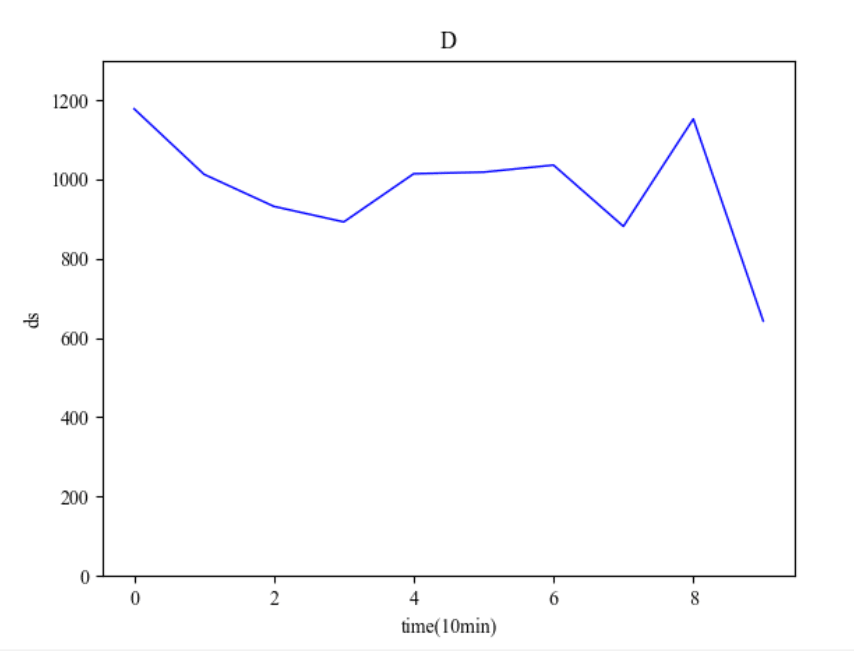
\includegraphics[width=\textwidth]{figures/d1.png}
			\caption{The Dispersion of the Position of the Players.}
			\label{fig:d1}
		\end{subfigure}%
		\begin{subfigure}[b]{0.5\textwidth}
			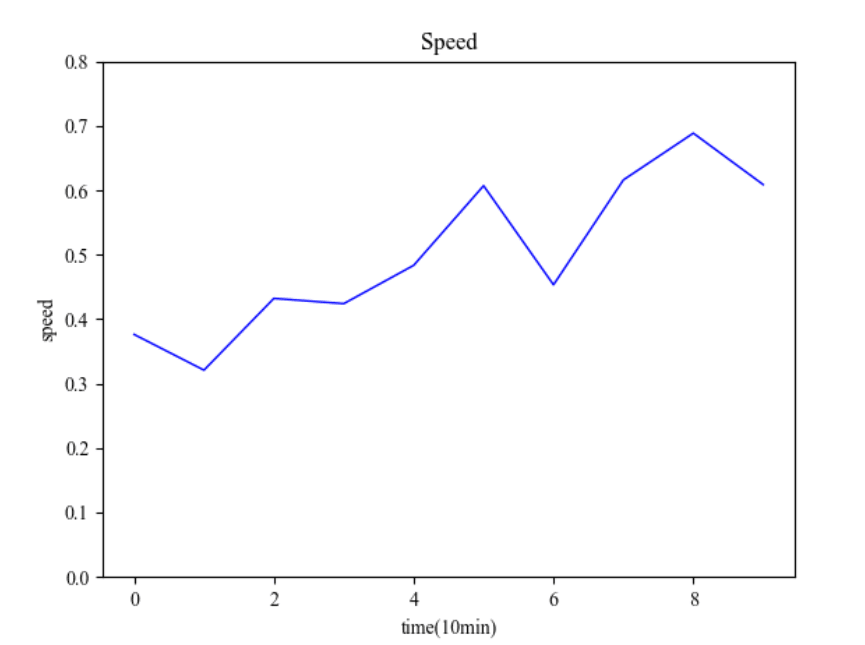
\includegraphics[width=\textwidth]{figures/s1.png}
			\caption{The Advance Speed.}
			\label{fig:s1}
		\end{subfigure}
		\caption{The Change of Network Centroid's Coordinates, the Dispersion of the Position of the Players around the Network Centroid And the Advance Speed over Time in a Game.}\label{fig:game}
	\end{figure}

	\begin{figure}[h]
		\centering
		\begin{subfigure}[b]{0.5\textwidth}
			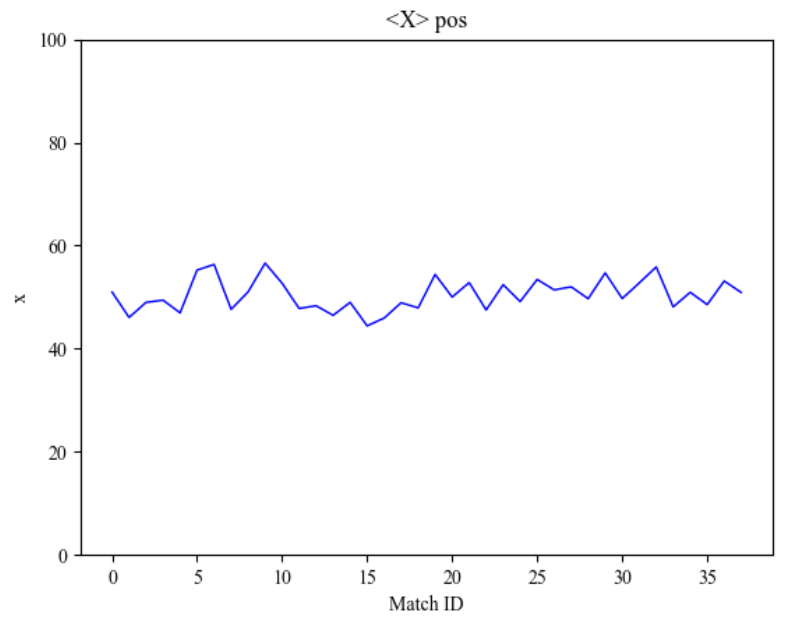
\includegraphics[width=\textwidth]{figures/xc2.png}
			\caption{The X-coordinate of the Network Centroid.}
			\label{fig:x2}
		\end{subfigure}%
		\begin{subfigure}[b]{0.5\textwidth}
			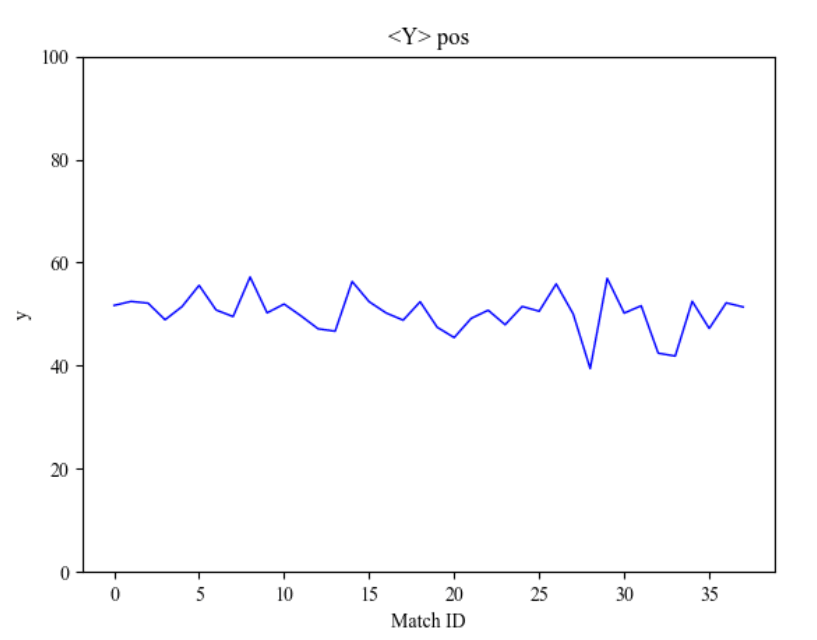
\includegraphics[width=\textwidth]{figures/yc2.png}
			\caption{The Y-coordinate of the Network Centroid.}
			\label{fig:y2}
		\end{subfigure}
		\begin{subfigure}[b]{0.5\textwidth}
			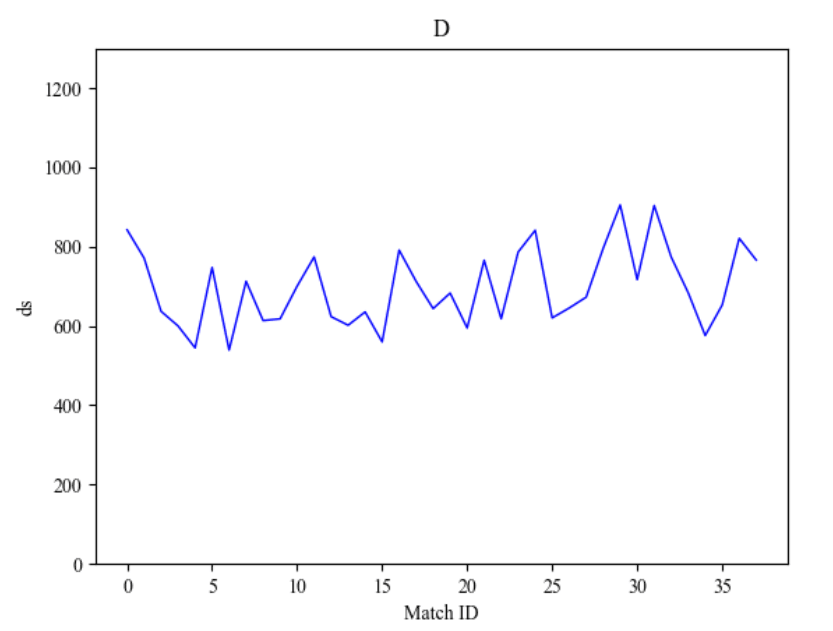
\includegraphics[width=\textwidth]{figures/d2.png}
			\caption{The Dispersion of the Position of the Players.}
			\label{fig:d2}
		\end{subfigure}%
		\begin{subfigure}[b]{0.5\textwidth}
			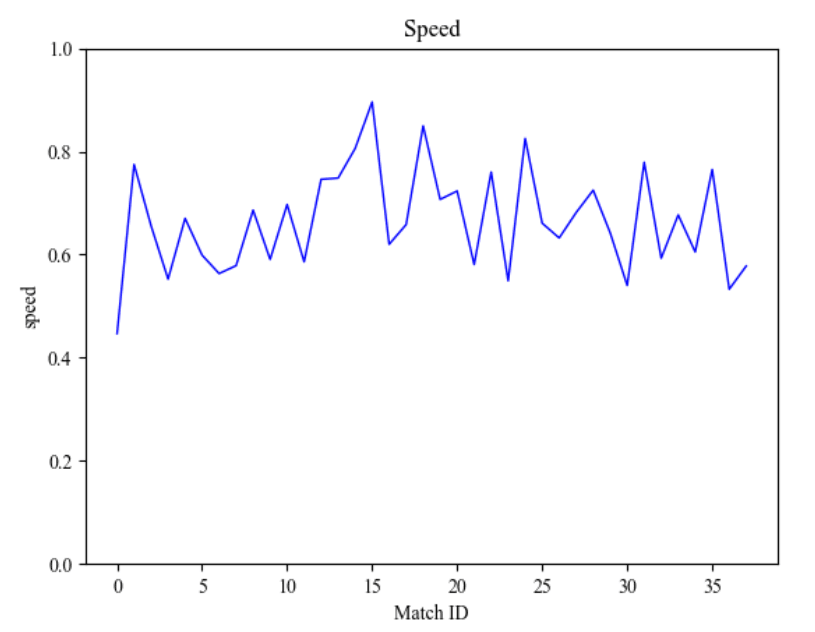
\includegraphics[width=\textwidth]{figures/s2.png}
			\caption{The Advance Speed.}
			\label{fig:s2}
		\end{subfigure}
		\caption{The Change of Network Centroid's Coordinates, the Dispersion of the Position of the Players around the Network Centroid And the Advance Speed over Games in the Entire Season.}\label{fig:season}
	\end{figure}
\subsection{Teamwork Indicators}
\section{Structural Strategies}
\subsection{Offensive tactics}
\begin{enumerate}[(1)]
	\item \textbf{Backcourt}.\par
	\qquad Outstanding team offenses are looking for opportunities and seizing opportunities to attack. Therefore, the strong team's ball possession rate is generally maintained at a high level. And the strong team's passing network can be seen, their defenders pass the most. A good player should seize the opportunities rather than afraid of waste of time. By passing each other back, grasping the ball can not only relieve the pressure, but also create good offensive opportunities. \par
	\qquad The back pass is often used in football games. It can not only play a tactical role in local cooperation, but also give strategic significance to the situation in the entire court. Offensively, by passing back the ball, you can flexibly grasp the offensive direction, adjust the rhythm of the game, and mobilize the opponent. Take advantage of the loopholes in the opponent's transfer to seek shooting opportunities and create conditions for scoring. Therefore, it is necessary to increase the proportion of guards transmitting the ball to each other and exercise precision and non-stealth.
	\begin{figure}[h]
		\centering
		\begin{subfigure}[b]{0.45\textwidth}
			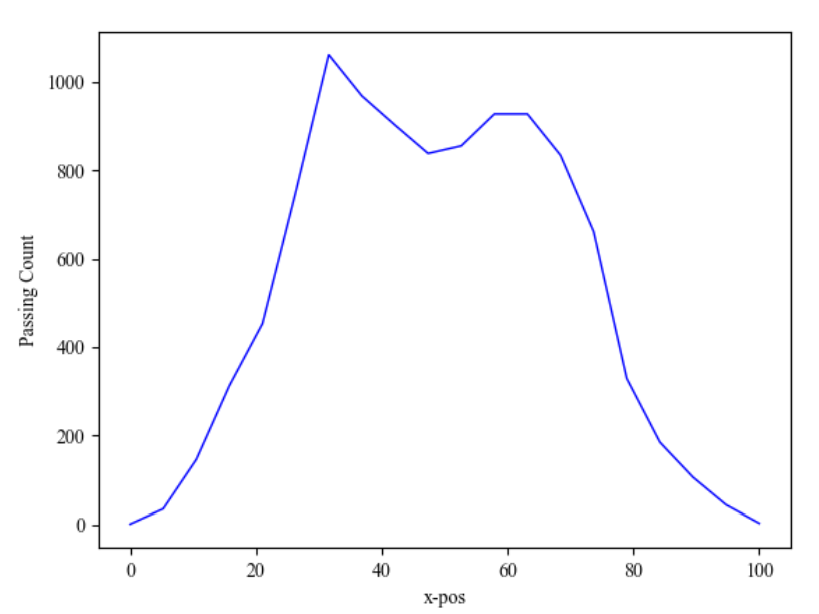
\includegraphics[width=\textwidth]{figures/backcourt.png}
			\caption{The team's number of passes changes with the x coordinate.}
			\label{fig:backcourt}
		\end{subfigure}
		\begin{subfigure}[b]{0.45\textwidth}
			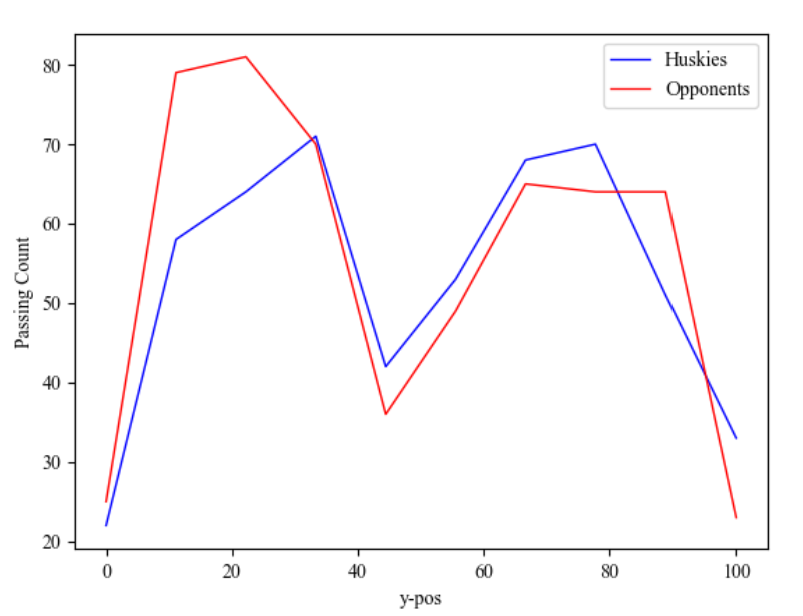
\includegraphics[width=\textwidth]{figures/backtofront_pos.png}
			\caption{The passing count of the passing in the middle and on the side. }
			\label{fig:back_to_front}
		\end{subfigure}
		\label{fig:passing_count}
		\caption{The passing count position.}
	\end{figure}
	\item \textbf{Continuous pass.}\par
	\qquad It can be seen from the data that triangle tactics are used the most and can also achieve good results. Continuous passes can allow opponents to run out of gear before they react, and they can excel without confrontation. Good passing coordination can even bypass the opponent's defensive line and enter the dangerous position for shooting. In the midfield, you can also use a straight pass to cooperate with the two-on-one. Therefore, it is necessary to increase the ability of forwards and wing centers to respond, and continuously forward the ball to make it easier for the forward to pass through the defense line of the opposing defender.
	\item \textbf{Sidewalk alternation.}\par
	\qquad Don't focus too much on the middle. Although the area of the middle is large and the angle is good, it is also the main force of the opponent's defense. So more opportunities are created in the sidewalks, and active crossovers can play an unexpected role. By analyzing the lost games of the Huskies, it can be seen that most of the opponents are active wing alternates to make it easy to dissolve the Husky's back line of defense. Therefore, for the purpose of learning from others, the front lines on the left and right should actively run without the ball to create opportunities for passing in the middle and communicate with each other. This can largely tear the defense of the team with poor defense line.
	\item \textbf{Short and long passes work together}\par
	\qquad After a large number of short passes, the sudden high ball often caught the opponent by surprise. The offensive player only needs to occupy the place in advance to easily tear the opponent's defensive line to bring the ball into the penalty area. The strong team's ball network can often see a large range of ball, which not only can make a sudden change in rhythm so that the opponent can not cope, and can easily send the ball to the opponent's penalty area.\par
	\qquad In addition, there is the forward's response and ability to grab positions. Being able to run to the ball in time is an important ability requirement for the forward. In addition to the large-scale Cross, another popular high kick in football today is long corner kicks. At this stage, long-distance corner kicks have become a key part of strong team tactics. If it is difficult to enter the penalty area, you can choose to win the corner by creating an opponent player out of bounds. Find opportunities to score in the long corner. At that time, the centers will all come up to help the forwards. This will be much easier than the striker's cooperation into the restricted area. Therefore, you should train long-distance conductive balls to increase the large-scale conductive balls in the network.
	\begin{figure}[htbp]
		\centering
		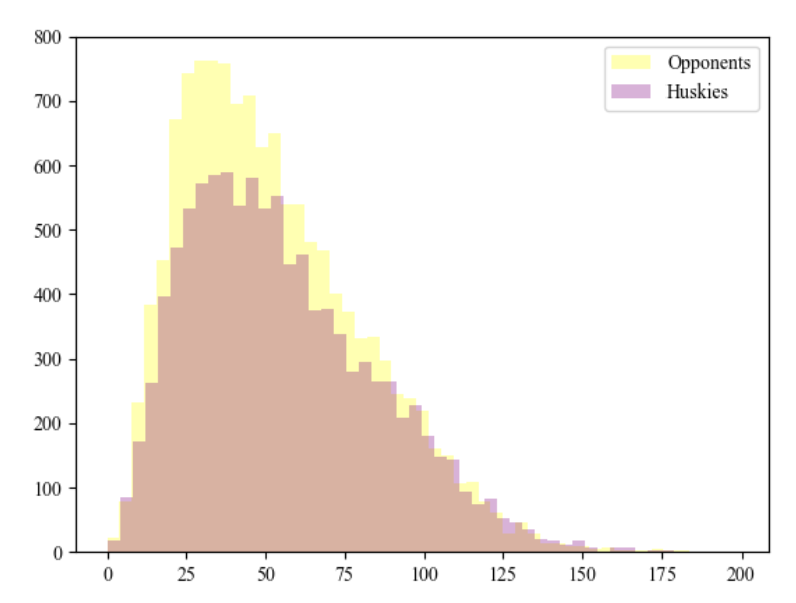
\includegraphics[width=0.5\textwidth]{figures/passing_cnt.png}
		\caption{The passing distance count for Huskies and the opponents. The opponents have more passings than Huskies and the average distance of passing is a bit smaller than  the Huskies.}
		\label{fig:passing_cnt}
	\end{figure}
	\item \textbf{Reduced Short Corners}\par
	\qquad Near the corner, the player quickly passed the ball to the forward teammate, and cooperated with the back pass to complete the shot. Short-kick corner kicks extend the time of the offense because they must be launched after the coordinated pass. While the same team members select positions, the opposing defensive players and goalkeepers' positions will be more accurate, thereby forming a good defensive formation. This is not conducive to grab a point attack. Therefore, in many cases, short corner kicks are issued quickly when the opponent's defensive position is not tight to gain a short-term advantage in time and space, and seek better passing points through passing. But at this stage, the strong teams' defense lines are very solid, so it is difficult to find such opportunities. Therefore the number of short corner kicks should be reduced.
\end{enumerate}
\section{Model Analysis}
\subsection{Sensitivity Analysis}
\subsection{Strengths and Weakness}
\section{Conclusion}

\bibliography{ref}
\newpage

\begin{appendices}


\end{appendices}

\end{document}
